% Options for packages loaded elsewhere
\PassOptionsToPackage{unicode}{hyperref}
\PassOptionsToPackage{hyphens}{url}
\PassOptionsToPackage{dvipsnames,svgnames,x11names}{xcolor}
%
\documentclass[
  letterpaper,
  DIV=11,
  numbers=noendperiod]{scrartcl}

\usepackage{amsmath,amssymb}
\usepackage{iftex}
\ifPDFTeX
  \usepackage[T1]{fontenc}
  \usepackage[utf8]{inputenc}
  \usepackage{textcomp} % provide euro and other symbols
\else % if luatex or xetex
  \usepackage{unicode-math}
  \defaultfontfeatures{Scale=MatchLowercase}
  \defaultfontfeatures[\rmfamily]{Ligatures=TeX,Scale=1}
\fi
\usepackage{lmodern}
\ifPDFTeX\else  
    % xetex/luatex font selection
\fi
% Use upquote if available, for straight quotes in verbatim environments
\IfFileExists{upquote.sty}{\usepackage{upquote}}{}
\IfFileExists{microtype.sty}{% use microtype if available
  \usepackage[]{microtype}
  \UseMicrotypeSet[protrusion]{basicmath} % disable protrusion for tt fonts
}{}
\makeatletter
\@ifundefined{KOMAClassName}{% if non-KOMA class
  \IfFileExists{parskip.sty}{%
    \usepackage{parskip}
  }{% else
    \setlength{\parindent}{0pt}
    \setlength{\parskip}{6pt plus 2pt minus 1pt}}
}{% if KOMA class
  \KOMAoptions{parskip=half}}
\makeatother
\usepackage{xcolor}
\setlength{\emergencystretch}{3em} % prevent overfull lines
\setcounter{secnumdepth}{5}
% Make \paragraph and \subparagraph free-standing
\ifx\paragraph\undefined\else
  \let\oldparagraph\paragraph
  \renewcommand{\paragraph}[1]{\oldparagraph{#1}\mbox{}}
\fi
\ifx\subparagraph\undefined\else
  \let\oldsubparagraph\subparagraph
  \renewcommand{\subparagraph}[1]{\oldsubparagraph{#1}\mbox{}}
\fi

\usepackage{color}
\usepackage{fancyvrb}
\newcommand{\VerbBar}{|}
\newcommand{\VERB}{\Verb[commandchars=\\\{\}]}
\DefineVerbatimEnvironment{Highlighting}{Verbatim}{commandchars=\\\{\}}
% Add ',fontsize=\small' for more characters per line
\usepackage{framed}
\definecolor{shadecolor}{RGB}{241,243,245}
\newenvironment{Shaded}{\begin{snugshade}}{\end{snugshade}}
\newcommand{\AlertTok}[1]{\textcolor[rgb]{0.68,0.00,0.00}{#1}}
\newcommand{\AnnotationTok}[1]{\textcolor[rgb]{0.37,0.37,0.37}{#1}}
\newcommand{\AttributeTok}[1]{\textcolor[rgb]{0.40,0.45,0.13}{#1}}
\newcommand{\BaseNTok}[1]{\textcolor[rgb]{0.68,0.00,0.00}{#1}}
\newcommand{\BuiltInTok}[1]{\textcolor[rgb]{0.00,0.23,0.31}{#1}}
\newcommand{\CharTok}[1]{\textcolor[rgb]{0.13,0.47,0.30}{#1}}
\newcommand{\CommentTok}[1]{\textcolor[rgb]{0.37,0.37,0.37}{#1}}
\newcommand{\CommentVarTok}[1]{\textcolor[rgb]{0.37,0.37,0.37}{\textit{#1}}}
\newcommand{\ConstantTok}[1]{\textcolor[rgb]{0.56,0.35,0.01}{#1}}
\newcommand{\ControlFlowTok}[1]{\textcolor[rgb]{0.00,0.23,0.31}{#1}}
\newcommand{\DataTypeTok}[1]{\textcolor[rgb]{0.68,0.00,0.00}{#1}}
\newcommand{\DecValTok}[1]{\textcolor[rgb]{0.68,0.00,0.00}{#1}}
\newcommand{\DocumentationTok}[1]{\textcolor[rgb]{0.37,0.37,0.37}{\textit{#1}}}
\newcommand{\ErrorTok}[1]{\textcolor[rgb]{0.68,0.00,0.00}{#1}}
\newcommand{\ExtensionTok}[1]{\textcolor[rgb]{0.00,0.23,0.31}{#1}}
\newcommand{\FloatTok}[1]{\textcolor[rgb]{0.68,0.00,0.00}{#1}}
\newcommand{\FunctionTok}[1]{\textcolor[rgb]{0.28,0.35,0.67}{#1}}
\newcommand{\ImportTok}[1]{\textcolor[rgb]{0.00,0.46,0.62}{#1}}
\newcommand{\InformationTok}[1]{\textcolor[rgb]{0.37,0.37,0.37}{#1}}
\newcommand{\KeywordTok}[1]{\textcolor[rgb]{0.00,0.23,0.31}{#1}}
\newcommand{\NormalTok}[1]{\textcolor[rgb]{0.00,0.23,0.31}{#1}}
\newcommand{\OperatorTok}[1]{\textcolor[rgb]{0.37,0.37,0.37}{#1}}
\newcommand{\OtherTok}[1]{\textcolor[rgb]{0.00,0.23,0.31}{#1}}
\newcommand{\PreprocessorTok}[1]{\textcolor[rgb]{0.68,0.00,0.00}{#1}}
\newcommand{\RegionMarkerTok}[1]{\textcolor[rgb]{0.00,0.23,0.31}{#1}}
\newcommand{\SpecialCharTok}[1]{\textcolor[rgb]{0.37,0.37,0.37}{#1}}
\newcommand{\SpecialStringTok}[1]{\textcolor[rgb]{0.13,0.47,0.30}{#1}}
\newcommand{\StringTok}[1]{\textcolor[rgb]{0.13,0.47,0.30}{#1}}
\newcommand{\VariableTok}[1]{\textcolor[rgb]{0.07,0.07,0.07}{#1}}
\newcommand{\VerbatimStringTok}[1]{\textcolor[rgb]{0.13,0.47,0.30}{#1}}
\newcommand{\WarningTok}[1]{\textcolor[rgb]{0.37,0.37,0.37}{\textit{#1}}}

\providecommand{\tightlist}{%
  \setlength{\itemsep}{0pt}\setlength{\parskip}{0pt}}\usepackage{longtable,booktabs,array}
\usepackage{calc} % for calculating minipage widths
% Correct order of tables after \paragraph or \subparagraph
\usepackage{etoolbox}
\makeatletter
\patchcmd\longtable{\par}{\if@noskipsec\mbox{}\fi\par}{}{}
\makeatother
% Allow footnotes in longtable head/foot
\IfFileExists{footnotehyper.sty}{\usepackage{footnotehyper}}{\usepackage{footnote}}
\makesavenoteenv{longtable}
\usepackage{graphicx}
\makeatletter
\def\maxwidth{\ifdim\Gin@nat@width>\linewidth\linewidth\else\Gin@nat@width\fi}
\def\maxheight{\ifdim\Gin@nat@height>\textheight\textheight\else\Gin@nat@height\fi}
\makeatother
% Scale images if necessary, so that they will not overflow the page
% margins by default, and it is still possible to overwrite the defaults
% using explicit options in \includegraphics[width, height, ...]{}
\setkeys{Gin}{width=\maxwidth,height=\maxheight,keepaspectratio}
% Set default figure placement to htbp
\makeatletter
\def\fps@figure{htbp}
\makeatother

% load packages
\usepackage{geometry}
\usepackage{xcolor}
\usepackage{eso-pic}
\usepackage{fancyhdr}
\usepackage{sectsty}
\usepackage{fontspec}
\usepackage{titlesec}

%% Set page size with a wider right margin
\geometry{a4paper, total={170mm,257mm}, left=20mm, top=20mm, bottom=20mm, right=50mm}

%% Let's define some colours
\definecolor{uniblue}{HTML}{003865}
\definecolor{burgundy}{HTML}{7D2239}
\definecolor{cobalt}{HTML}{005C8A}
\definecolor{lavender}{HTML}{5B4D94}
\definecolor{leaf}{HTML}{006630}
\definecolor{moss}{HTML}{385A4F}
\definecolor{pillarbox}{HTML}{B30C00}
\definecolor{rust}{HTML}{9A3A06}
\definecolor{sandstone}{HTML}{52473B}
\definecolor{skyblue}{HTML}{005398}
\definecolor{slate}{HTML}{4F5961}
\definecolor{thistle}{HTML}{951272}

%\definecolor{light}{HTML}{E6E6FA} % original from template - redefined below as uni blue at 10 percent:
\colorlet{light}{uniblue!10}
%\definecolor{highlight}{HTML}{800080} % original from template - redefined below as uni's skyblue:
\colorlet{highlight}{skyblue}
%\definecolor{dark}{HTML}{330033} % original from template - redefined below as uni blue at 100 percent:
\colorlet{dark}{uniblue}

%% Let's add the border on the right hand side 
\AddToShipoutPicture{% 
    \AtPageLowerLeft{% 
        \put(\LenToUnit{\dimexpr\paperwidth-3cm},0){% 
            \color{light}\rule{3cm}{\LenToUnit\paperheight}%
          }%
     }%
     % logo
    \AtPageLowerLeft{% start the bar at the bottom right of the page
        \put(\LenToUnit{\dimexpr\paperwidth-2.25cm},27.2cm){% move it to the top right
            \color{light}
\includegraphics[width=2.25cm]{_extensions/nrennie/PrettyPDF/uni_logo_boxed.jpg}
          }%
     }%
}

%% Style the page number
\fancypagestyle{mystyle}{
  \fancyhf{}
  \renewcommand\headrulewidth{0pt}
  \fancyfoot[R]{\thepage}
  \fancyfootoffset{3.5cm}
}
\setlength{\footskip}{20pt}

%% style the chapter/section fonts
\chapterfont{\color{uniblue}\fontsize{20}{16.8}\selectfont}
\sectionfont{\color{uniblue}\fontsize{20}{16.8}\selectfont}
\subsectionfont{\color{skyblue}\fontsize{14}{16.8}\selectfont}
\titleformat{\subsection}
  {\color{uniblue!90}\sffamily\Large\bfseries}{\thesubsection}{1em}{}[{\titlerule[0.8pt]}]
\subsubsectionfont{\color{cobalt}}

\renewcommand\thesection{\color{slate}\arabic{section}}
  
% left align title
\makeatletter
\renewcommand{\maketitle}{\bgroup\setlength{\parindent}{0pt}
\begin{flushleft}
  {\color{uniblue}\sffamily\huge\textbf{\@title}} \vspace{0.3cm} \newline
  {\Large {\@subtitle}} \newline
  \@author
\end{flushleft}\egroup
}
\makeatother

%% Use some custom fonts
\setsansfont{Ubuntu}[
    Path=_extensions/nrennie/PrettyPDF/Ubuntu/,
    Scale=0.9,
    Extension = .ttf,
    UprightFont=*-Regular,
    BoldFont=*-Bold,
    ItalicFont=*-Italic,
    ]

\setmainfont{Ubuntu}[
    Path=_extensions/nrennie/PrettyPDF/Ubuntu/,
    Scale=0.9,
    Extension = .ttf,
    UprightFont=*-Regular,
    BoldFont=*-Bold,
    ItalicFont=*-Italic,
    ]
\KOMAoption{captions}{tableheading}
\makeatletter
\@ifpackageloaded{tcolorbox}{}{\usepackage[skins,breakable]{tcolorbox}}
\@ifpackageloaded{fontawesome5}{}{\usepackage{fontawesome5}}
\definecolor{quarto-callout-color}{HTML}{909090}
\definecolor{quarto-callout-note-color}{HTML}{0758E5}
\definecolor{quarto-callout-important-color}{HTML}{CC1914}
\definecolor{quarto-callout-warning-color}{HTML}{EB9113}
\definecolor{quarto-callout-tip-color}{HTML}{00A047}
\definecolor{quarto-callout-caution-color}{HTML}{FC5300}
\definecolor{quarto-callout-color-frame}{HTML}{acacac}
\definecolor{quarto-callout-note-color-frame}{HTML}{4582ec}
\definecolor{quarto-callout-important-color-frame}{HTML}{d9534f}
\definecolor{quarto-callout-warning-color-frame}{HTML}{f0ad4e}
\definecolor{quarto-callout-tip-color-frame}{HTML}{02b875}
\definecolor{quarto-callout-caution-color-frame}{HTML}{fd7e14}
\makeatother
\makeatletter
\@ifpackageloaded{caption}{}{\usepackage{caption}}
\AtBeginDocument{%
\ifdefined\contentsname
  \renewcommand*\contentsname{Table of contents}
\else
  \newcommand\contentsname{Table of contents}
\fi
\ifdefined\listfigurename
  \renewcommand*\listfigurename{List of Figures}
\else
  \newcommand\listfigurename{List of Figures}
\fi
\ifdefined\listtablename
  \renewcommand*\listtablename{List of Tables}
\else
  \newcommand\listtablename{List of Tables}
\fi
\ifdefined\figurename
  \renewcommand*\figurename{Figure}
\else
  \newcommand\figurename{Figure}
\fi
\ifdefined\tablename
  \renewcommand*\tablename{Table}
\else
  \newcommand\tablename{Table}
\fi
}
\@ifpackageloaded{float}{}{\usepackage{float}}
\floatstyle{ruled}
\@ifundefined{c@chapter}{\newfloat{codelisting}{h}{lop}}{\newfloat{codelisting}{h}{lop}[chapter]}
\floatname{codelisting}{Listing}
\newcommand*\listoflistings{\listof{codelisting}{List of Listings}}
\makeatother
\makeatletter
\makeatother
\makeatletter
\@ifpackageloaded{caption}{}{\usepackage{caption}}
\@ifpackageloaded{subcaption}{}{\usepackage{subcaption}}
\makeatother
\makeatletter
\@ifpackageloaded{tcolorbox}{}{\usepackage[skins,breakable]{tcolorbox}}
\makeatother
\makeatletter
\@ifundefined{shadecolor}{\definecolor{shadecolor}{rgb}{.97, .97, .97}}{}
\makeatother
\makeatletter
\@ifundefined{codebgcolor}{\definecolor{codebgcolor}{named}{light}}{}
\makeatother
\makeatletter
\ifdefined\Shaded\renewenvironment{Shaded}{\begin{tcolorbox}[frame hidden, colback={codebgcolor}, breakable, enhanced, sharp corners, boxrule=0pt]}{\end{tcolorbox}}\fi
\makeatother
\ifLuaTeX
  \usepackage{selnolig}  % disable illegal ligatures
\fi
\usepackage{bookmark}

\IfFileExists{xurl.sty}{\usepackage{xurl}}{} % add URL line breaks if available
\urlstyle{same} % disable monospaced font for URLs
\hypersetup{
  pdftitle={Extra material},
  colorlinks=true,
  linkcolor={highlight},
  filecolor={Maroon},
  citecolor={Blue},
  urlcolor={highlight},
  pdfcreator={LaTeX via pandoc}}

\title{Extra material}
\author{}
\date{}

\begin{document}
\maketitle

\pagestyle{mystyle}

\section{Working with dates and
times}\label{working-with-dates-and-times}

Working with date-time data in R can be challenging due to the
unintuitive and inconsistent commands across different date-time
objects. Additionally, managing things like time zones, leap days, and
daylight saving time can be tricky since R doesn't always handle these
well. The \texttt{lubridate} and \texttt{hms} packages (loaded as part
of \texttt{tideverse}) simplify date-time operations in R, making it
easier to perform common tasks and enabling functionalities that R's
base capabilities do not support. Unfortunately, we don't have enough
time to cover all the details in this session. Instead, we will only
give short introduction on how to work and manipulate date and time
variables in R using the \texttt{lubridate} and \texttt{hms} packages.
But if you want to learn more please have a look at the
\href{https://r4ds.hadley.nz/datetimes}{R for Data Science} ebook.

First, what do we mean by Date/Time data? well, when we speak of
Date/Time data we are mainly referring to three data types:

\begin{enumerate}
\def\labelenumi{\arabic{enumi}.}
\item
  \textbf{Date} - a variable containing only the date when an
  observation was made (e.g.~2024-07-12). More formally, it is a day
  stored as the number of days since 1970-01-01
\item
  \textbf{Time} - a variable containing only the time when an
  observation was made (e.g.~18:15:00). Formally , the number of seconds
  since 00:00:00
\item
  \textbf{Date \& Time} - combination of both the date and time
  (e.g.~2024-07-12 18:15:00). Formally, is a point on the timeline,
  stored as the number of seconds since 1970-01-01 00:00:00 UTC
\end{enumerate}

There are several ways in which Date-time variables can be created. Here
are some examples:

\begin{Shaded}
\begin{Highlighting}[]
\CommentTok{\# Example 1: string input with date Y/M/D format}
\FunctionTok{ymd}\NormalTok{(}\StringTok{"2017{-}01{-}31"}\NormalTok{)}
\end{Highlighting}
\end{Shaded}

\begin{verbatim}
[1] "2017-01-31"
\end{verbatim}

\begin{Shaded}
\begin{Highlighting}[]
\CommentTok{\# Example 2: string input with date M/D/Y format}
\FunctionTok{mdy}\NormalTok{(}\StringTok{"January 31st, 2017"}\NormalTok{)}
\end{Highlighting}
\end{Shaded}

\begin{verbatim}
[1] "2017-01-31"
\end{verbatim}

\begin{Shaded}
\begin{Highlighting}[]
\CommentTok{\# Example 3: string input with date D/M/Y format}
\FunctionTok{dmy}\NormalTok{(}\StringTok{"31{-}Jan{-}2017"}\NormalTok{)}
\end{Highlighting}
\end{Shaded}

\begin{verbatim}
[1] "2017-01-31"
\end{verbatim}

\begin{Shaded}
\begin{Highlighting}[]
\CommentTok{\# Example 4: numeric input with date M/D/Y format}
\FunctionTok{mdy}\NormalTok{(}\DecValTok{07082016}\NormalTok{)}
\end{Highlighting}
\end{Shaded}

\begin{verbatim}
[1] "2016-07-08"
\end{verbatim}

\begin{Shaded}
\begin{Highlighting}[]
\CommentTok{\# Examples 5: string input with time H:M formate}
\FunctionTok{hm}\NormalTok{(}\StringTok{"20:11"}\NormalTok{)}
\end{Highlighting}
\end{Shaded}

\begin{verbatim}
[1] "20H 11M 0S"
\end{verbatim}

\begin{Shaded}
\begin{Highlighting}[]
\CommentTok{\# Example 6:  string input with date{-}time D/M/Y H:M:S}
\FunctionTok{ymd\_hms}\NormalTok{(}\StringTok{"2017{-}01{-}31 20:11:59"}\NormalTok{)}
\end{Highlighting}
\end{Shaded}

\begin{verbatim}
[1] "2017-01-31 20:11:59 UTC"
\end{verbatim}

In this session, instead of creating data-time variables by ourselves,
we will focus on already existing Date/Time Data. Let's look at some of
the date-time variables in the \texttt{flights} data set, namely the
scheduled departure dates and times:

\section{Output}

\begin{verbatim}
# A tibble: 336,776 x 5
    year month   day  hour minute
   <int> <int> <int> <dbl>  <dbl>
 1  2013     1     1     5     15
 2  2013     1     1     5     29
 3  2013     1     1     5     40
 4  2013     1     1     5     45
 5  2013     1     1     6      0
 6  2013     1     1     5     58
 7  2013     1     1     6      0
 8  2013     1     1     6      0
 9  2013     1     1     6      0
10  2013     1     1     6      0
# i 336,766 more rows
\end{verbatim}

\section{R-Code}

\begin{Shaded}
\begin{Highlighting}[]
\NormalTok{flights\_dep }\OtherTok{\textless{}{-}}\NormalTok{ flights }\SpecialCharTok{\%\textgreater{}\%}
  \FunctionTok{select}\NormalTok{(year, month, day, hour, minute)}
\NormalTok{flights\_dep}
\end{Highlighting}
\end{Shaded}

Instead of having separate date-time variables spread across different
columns, we can use the \texttt{make\_date()} or
\texttt{make\_datetime()}functions to create new date and date-time
variables respectively:

\begin{Shaded}
\begin{Highlighting}[]
\NormalTok{flights\_dep }\OtherTok{\textless{}{-}}\NormalTok{ flights\_dep }\SpecialCharTok{\%\textgreater{}\%}
    \FunctionTok{mutate}\NormalTok{(}\AttributeTok{departure\_time =} \FunctionTok{make\_datetime}\NormalTok{(year, month, day, hour, minute),}
           \AttributeTok{departure\_date =} \FunctionTok{make\_date}\NormalTok{(year, month, day))}
\NormalTok{flights\_dep}
\end{Highlighting}
\end{Shaded}

\begin{verbatim}
# A tibble: 336,776 x 7
    year month   day  hour minute departure_time      departure_date
   <int> <int> <int> <dbl>  <dbl> <dttm>              <date>        
 1  2013     1     1     5     15 2013-01-01 05:15:00 2013-01-01    
 2  2013     1     1     5     29 2013-01-01 05:29:00 2013-01-01    
 3  2013     1     1     5     40 2013-01-01 05:40:00 2013-01-01    
 4  2013     1     1     5     45 2013-01-01 05:45:00 2013-01-01    
 5  2013     1     1     6      0 2013-01-01 06:00:00 2013-01-01    
 6  2013     1     1     5     58 2013-01-01 05:58:00 2013-01-01    
 7  2013     1     1     6      0 2013-01-01 06:00:00 2013-01-01    
 8  2013     1     1     6      0 2013-01-01 06:00:00 2013-01-01    
 9  2013     1     1     6      0 2013-01-01 06:00:00 2013-01-01    
10  2013     1     1     6      0 2013-01-01 06:00:00 2013-01-01    
# i 336,766 more rows
\end{verbatim}

We then can visualize the distribution of the scheduled departure times
across the year with ggplot by adding a \texttt{geom\_freqpoly()} layer
(which is similar to an histogram where the counts are displayed with
lines instead of bars). Note that when you use date-times in a numeric
context (like in a histogram), a binwidth of 1 is equivalent to 1
second, so a binwidth of 86400 is equivalent to one day.

\begin{Shaded}
\begin{Highlighting}[]
\NormalTok{flights\_dep }\SpecialCharTok{\%\textgreater{}\%}
  \FunctionTok{ggplot}\NormalTok{(}\FunctionTok{aes}\NormalTok{(}\AttributeTok{x =}\NormalTok{ departure\_time)) }\SpecialCharTok{+}
  \FunctionTok{geom\_freqpoly}\NormalTok{(}\AttributeTok{binwidth =} \DecValTok{86400}\NormalTok{) }\CommentTok{\# 86400 seconds = 1 day}
\end{Highlighting}
\end{Shaded}

\begin{center}
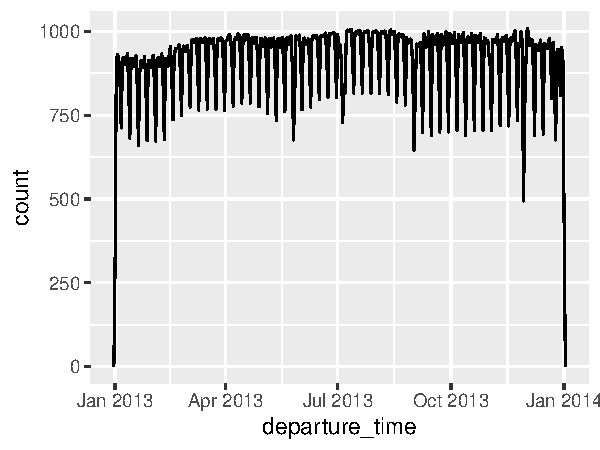
\includegraphics{tutorial_files/figure-pdf/unnamed-chunk-6-1.pdf}
\end{center}

Likewise, if were interested in the distribution of the scheduled
departures for a given day:

\begin{Shaded}
\begin{Highlighting}[]
\NormalTok{flights\_dep }\SpecialCharTok{\%\textgreater{}\%}
  \FunctionTok{filter}\NormalTok{(departure\_date }\SpecialCharTok{==} \FunctionTok{ymd}\NormalTok{(}\DecValTok{20130102}\NormalTok{)) }\SpecialCharTok{\%\textgreater{}\%}
  \FunctionTok{ggplot}\NormalTok{(}\FunctionTok{aes}\NormalTok{(}\AttributeTok{x =}\NormalTok{ departure\_time)) }\SpecialCharTok{+}
  \FunctionTok{geom\_freqpoly}\NormalTok{(}\AttributeTok{binwidth =} \DecValTok{600}\NormalTok{) }\CommentTok{\# 600 s = 10 minutes}
\end{Highlighting}
\end{Shaded}

\begin{center}
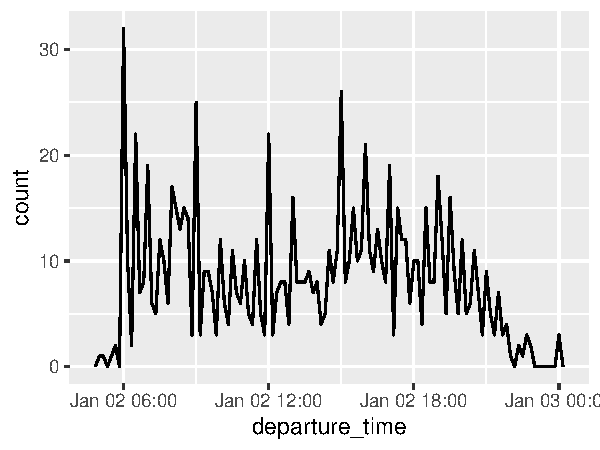
\includegraphics{tutorial_files/figure-pdf/unnamed-chunk-7-1.pdf}
\end{center}

In here, \texttt{binwidth\ =\ 600} means we are clumping all flights
within each 10 minutes (600 s) together into one single data point in
our frequency polygon.

Now, notice that in the original \texttt{flights} data set, the hour and
minute of the actual departure (\texttt{dep\_time}) and arrival times
(\texttt{arr\_time}) are encoded together into a single integer. Let
make a function that sets the actual times in a sensible format:

\begin{Shaded}
\begin{Highlighting}[]
\NormalTok{make\_datetime\_flights }\OtherTok{\textless{}{-}} \ControlFlowTok{function}\NormalTok{(year, month, day, time) \{}
\NormalTok{  hour }\OtherTok{\textless{}{-}} \FunctionTok{case\_when}\NormalTok{(}
      \FunctionTok{nchar}\NormalTok{(time)}\SpecialCharTok{==} \DecValTok{1} \SpecialCharTok{\textasciitilde{}}\NormalTok{ time  }\SpecialCharTok{\%/\%}\DecValTok{1}\NormalTok{,}
      \FunctionTok{nchar}\NormalTok{(time)}\SpecialCharTok{==} \DecValTok{2} \SpecialCharTok{\textasciitilde{}}\NormalTok{ time  }\SpecialCharTok{\%/\%}\DecValTok{10}\NormalTok{,}
      \AttributeTok{.default =}\NormalTok{  time  }\SpecialCharTok{\%/\%}\DecValTok{100}
\NormalTok{    )}

\NormalTok{  min }\OtherTok{\textless{}{-}} \FunctionTok{case\_when}\NormalTok{(}
      \FunctionTok{nchar}\NormalTok{(time)}\SpecialCharTok{==} \DecValTok{1} \SpecialCharTok{\textasciitilde{}}\NormalTok{ time  }\SpecialCharTok{\%\%}\DecValTok{1}\NormalTok{,}
      \FunctionTok{nchar}\NormalTok{(time)}\SpecialCharTok{==} \DecValTok{2} \SpecialCharTok{\textasciitilde{}}\NormalTok{ time  }\SpecialCharTok{\%\%}\DecValTok{10}\NormalTok{,}
      \AttributeTok{.default =}\NormalTok{  time  }\SpecialCharTok{\%\%}\DecValTok{100}
\NormalTok{    )}
  \FunctionTok{make\_datetime}\NormalTok{(year, month, day, hour, min)}
\NormalTok{\}}
\end{Highlighting}
\end{Shaded}

The new \texttt{make\_datetime\_flights()} function we just created
separates the hour and minute of a given HM input and pass it on to
\texttt{make\_datetime} function. This is achieved by using a vectorized
\texttt{case\_when} argument based on the number of characters in the
integer that uses the \texttt{\%/\%} or\texttt{\%\%} operator to find
(or discards accordingly) the remainder of an integer division to obtain
the hour and minute components (e.g.~\texttt{951\ \%/\%\ 100} and
\texttt{951\ \%\%\ 100} splits the entry \texttt{951} into 9 and 51
(9:15 am once converted to time-date data) while \texttt{15\ \%/\%\ 10}
and \texttt{15\ \%\%\ 10} and gives 1 and 5 (equivalent to 1:05 am in
date-time format) .

\begin{Shaded}
\begin{Highlighting}[]
\NormalTok{flights\_dt }\OtherTok{\textless{}{-}}\NormalTok{ flights }\SpecialCharTok{\%\textgreater{}\%}
  \FunctionTok{filter}\NormalTok{(}\SpecialCharTok{!}\FunctionTok{is.na}\NormalTok{(dep\_time), }\SpecialCharTok{!}\FunctionTok{is.na}\NormalTok{(arr\_time)) }\SpecialCharTok{\%\textgreater{}\%}
  \FunctionTok{mutate}\NormalTok{(}
    \AttributeTok{dep\_time =} \FunctionTok{make\_datetime\_flights}\NormalTok{(year, month, day, dep\_time),}
    \AttributeTok{arr\_time =} \FunctionTok{make\_datetime\_flights}\NormalTok{(year, month, day, arr\_time),}
    \AttributeTok{sched\_dep\_time =} \FunctionTok{make\_datetime\_flights}\NormalTok{(year, month, day, sched\_dep\_time),}
    \AttributeTok{sched\_arr\_time =} \FunctionTok{make\_datetime\_flights}\NormalTok{(year, month, day, sched\_arr\_time)}
\NormalTok{  )}

\NormalTok{flights\_dt }\SpecialCharTok{\%\textgreater{}\%}
  \FunctionTok{select}\NormalTok{(dep\_time,arr\_time,sched\_dep\_time,sched\_arr\_time) }\SpecialCharTok{\%\textgreater{}\%}
  \FunctionTok{slice}\NormalTok{(}\DecValTok{1}\SpecialCharTok{:}\DecValTok{3}\NormalTok{)}
\end{Highlighting}
\end{Shaded}

\begin{verbatim}
# A tibble: 3 x 4
  dep_time            arr_time            sched_dep_time     
  <dttm>              <dttm>              <dttm>             
1 2013-01-01 05:17:00 2013-01-01 08:30:00 2013-01-01 05:15:00
2 2013-01-01 05:33:00 2013-01-01 08:50:00 2013-01-01 05:29:00
3 2013-01-01 05:42:00 2013-01-01 09:23:00 2013-01-01 05:40:00
# i 1 more variable: sched_arr_time <dttm>
\end{verbatim}

\subsection{Extracting individual date-time
components}\label{extracting-individual-date-time-components}

The \texttt{lubridate} package also provide us with different tools for
extracting specific components from date-time objects (e.g.~year, month,
hours, minutes, etc). Suppose we are interested in finding out which day
of the week each flight took place. The \texttt{wday()} functions allow
us to extract the numeric entry of the day of the week, by including the
argument \texttt{label\ =TRUE}, we can also print the name of the
weekday as the output

\begin{Shaded}
\begin{Highlighting}[]
\NormalTok{flights\_dt }\SpecialCharTok{\%\textgreater{}\%}
   \FunctionTok{select}\NormalTok{(dep\_time,arr\_time,sched\_dep\_time,sched\_arr\_time) }\SpecialCharTok{\%\textgreater{}\%}
  \FunctionTok{mutate}\NormalTok{(}\AttributeTok{weekday =} \FunctionTok{wday}\NormalTok{(dep\_time,}\AttributeTok{label=}\ConstantTok{TRUE}\NormalTok{)) }\SpecialCharTok{\%\textgreater{}\%}
  \FunctionTok{slice\_sample}\NormalTok{(}\AttributeTok{n=}\DecValTok{5}\NormalTok{)}
\end{Highlighting}
\end{Shaded}

\begin{verbatim}
# A tibble: 5 x 5
  dep_time            arr_time            sched_dep_time     
  <dttm>              <dttm>              <dttm>             
1 2013-05-18 04:59:00 2013-05-18 06:38:00 2013-05-18 05:00:00
2 2013-04-04 07:43:00 2013-04-04 10:29:00 2013-04-04 07:29:00
3 2013-03-18 18:33:00 2013-03-18 21:57:00 2013-03-18 18:29:00
4 2013-04-19 18:35:00 2013-04-19 21:32:00 2013-04-19 18:29:00
5 2013-04-05 07:57:00 2013-04-05 10:09:00 2013-04-05 08:04:00
# i 2 more variables: sched_arr_time <dttm>, weekday <ord>
\end{verbatim}

Here are some more few examples of helper functions that allow you to
extract individual date-time components:

\begin{Shaded}
\begin{Highlighting}[]
\NormalTok{datetime }\OtherTok{\textless{}{-}} \FunctionTok{ymd\_hms}\NormalTok{(}\StringTok{"2026{-}07{-}08 12:34:56"}\NormalTok{)}

\FunctionTok{year}\NormalTok{(datetime)}
\end{Highlighting}
\end{Shaded}

\begin{verbatim}
[1] 2026
\end{verbatim}

\begin{Shaded}
\begin{Highlighting}[]
\FunctionTok{month}\NormalTok{(datetime,}\AttributeTok{label =} \ConstantTok{TRUE}\NormalTok{)}
\end{Highlighting}
\end{Shaded}

\begin{verbatim}
[1] Jul
12 Levels: Jan < Feb < Mar < Apr < May < Jun < Jul < Aug < Sep < ... < Dec
\end{verbatim}

\begin{Shaded}
\begin{Highlighting}[]
\FunctionTok{day}\NormalTok{(datetime)}
\end{Highlighting}
\end{Shaded}

\begin{verbatim}
[1] 8
\end{verbatim}

\begin{Shaded}
\begin{Highlighting}[]
\FunctionTok{hour}\NormalTok{(datetime)}
\end{Highlighting}
\end{Shaded}

\begin{verbatim}
[1] 12
\end{verbatim}

\begin{Shaded}
\begin{Highlighting}[]
\FunctionTok{minute}\NormalTok{(datetime)}
\end{Highlighting}
\end{Shaded}

\begin{verbatim}
[1] 34
\end{verbatim}

\begin{tcolorbox}[enhanced jigsaw, bottomtitle=1mm, bottomrule=.15mm, colframe=quarto-callout-warning-color-frame, opacitybacktitle=0.6, leftrule=.75mm, title={Task}, breakable, titlerule=0mm, coltitle=black, rightrule=.15mm, toptitle=1mm, arc=.35mm, colback=white, opacityback=0, left=2mm, toprule=.15mm, colbacktitle=quarto-callout-warning-color!10!white]

Can you make a plot showing how does the distribution of flight times
within a day change over the course of the year? i.e., how many flights
have taken off by each hour. Comment on the patterns

Take a hint

Within a day, we want to observe how the flight times differ. This means
we should look at how flight times differ by the hour (i.e how many
flights are taking off at every hour of the day). You can use the
\texttt{hour()} function to extract the hours for every departure time
and then count (using \texttt{summarize()}) how many flights have taken
off by each hour. You can visualize the trend using \texttt{geom\_line}
in ggplot.

Click here to see the solution

\begin{Shaded}
\begin{Highlighting}[]
\NormalTok{flights\_dt }\SpecialCharTok{\%\textgreater{}\%}
  \FunctionTok{mutate}\NormalTok{(}\AttributeTok{hour =} \FunctionTok{hour}\NormalTok{(dep\_time)) }\SpecialCharTok{\%\textgreater{}\%}
  \FunctionTok{summarize}\NormalTok{(}\AttributeTok{numflights\_per\_hour =} \FunctionTok{n}\NormalTok{(),}\AttributeTok{.by=}\NormalTok{ hour)}\SpecialCharTok{\%\textgreater{}\%}
  \FunctionTok{ggplot}\NormalTok{(}\FunctionTok{aes}\NormalTok{(}\AttributeTok{x =}\NormalTok{ hour, }\AttributeTok{y =}\NormalTok{ numflights\_per\_hour)) }\SpecialCharTok{+}
    \FunctionTok{geom\_line}\NormalTok{() }\SpecialCharTok{+}
  \FunctionTok{labs}\NormalTok{(}\AttributeTok{y=}\StringTok{"number of flights per hour"}\NormalTok{,}\AttributeTok{x =} \StringTok{"hour"}\NormalTok{)}
\end{Highlighting}
\end{Shaded}

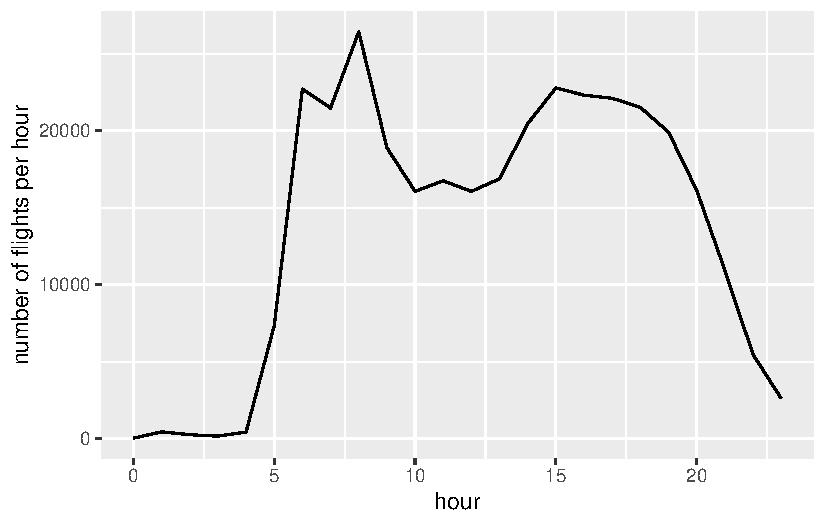
\includegraphics{tutorial_files/figure-pdf/unnamed-chunk-12-1.pdf}

We can see there is a peak of flights around 8am, a dip in flights from
10am-12pm, and then a drop off in number of flights past 7pm.

\end{tcolorbox}

\begin{tcolorbox}[enhanced jigsaw, bottomtitle=1mm, bottomrule=.15mm, colframe=quarto-callout-warning-color-frame, opacitybacktitle=0.6, leftrule=.75mm, title={Task}, breakable, titlerule=0mm, coltitle=black, rightrule=.15mm, toptitle=1mm, arc=.35mm, colback=white, opacityback=0, left=2mm, toprule=.15mm, colbacktitle=quarto-callout-warning-color!10!white]

Find out on what day of the week should you leave if you want to
minimise the chance of a delay?

Take a hint

To find the days of the week that have the lowest average delay, first
you need to assign a day to each observation using \texttt{wday()}. You
can then use \texttt{summarize()} and group by the the day of the week
to find the average delay time for each day of the week.

Click here to see the solution

\begin{Shaded}
\begin{Highlighting}[]
\NormalTok{flights\_dt }\SpecialCharTok{\%\textgreater{}\%}
  \FunctionTok{mutate}\NormalTok{(}\AttributeTok{wday =} \FunctionTok{wday}\NormalTok{(sched\_dep\_time, }\AttributeTok{label =} \ConstantTok{TRUE}\NormalTok{)) }\SpecialCharTok{\%\textgreater{}\%}
  \FunctionTok{group\_by}\NormalTok{(wday) }\SpecialCharTok{\%\textgreater{}\%}
  \FunctionTok{summarize}\NormalTok{ ( }\AttributeTok{avg\_dep\_delay\_week =} \FunctionTok{mean}\NormalTok{(dep\_delay, }\AttributeTok{na.rm =} \ConstantTok{TRUE}\NormalTok{),}
              \AttributeTok{avg\_arr\_delay\_week =} \FunctionTok{mean}\NormalTok{(arr\_delay, }\AttributeTok{na.rm =} \ConstantTok{TRUE}\NormalTok{)) }\SpecialCharTok{\%\textgreater{}\%}
  \FunctionTok{slice\_min}\NormalTok{(avg\_dep\_delay\_week,}\AttributeTok{n=}\DecValTok{1}\NormalTok{)}
\end{Highlighting}
\end{Shaded}

\begin{verbatim}
# A tibble: 1 x 3
  wday  avg_dep_delay_week avg_arr_delay_week
  <ord>              <dbl>              <dbl>
1 Sat                 7.62              -1.45
\end{verbatim}

\begin{Shaded}
\begin{Highlighting}[]
\CommentTok{\# Saturday has the lowest average delay at 7.61, and on average the flights even arrive earlier than expected!}
\end{Highlighting}
\end{Shaded}

We can see there is a peak of flights around 8am, a dip in flights from
10am-12pm, and then a drop off in number of flights past 7pm.

\end{tcolorbox}

\subsection{Time intervals, durations and
periods}\label{time-intervals-durations-and-periods}

Now that we have seen a few examples of R's date-time data structures,
lets look into some of the time span classes.

\begin{itemize}
\tightlist
\item
  Duration: exact number of seconds.
\item
  Periods: human units like weeks and months.
\item
  Intervals: a time span defined by a start and end point.
\end{itemize}

Duration is simply defined by the exact amount of time between two time
events. It does not consider what these two events are in terms
of,e.g.~calendar years or time zone (so things like leap years would be
ignored), and the output is shown in seconds. For example, say we want
to manually compute the departure delays in the \texttt{flights} data
set (we will use the \texttt{flights\_dt} data frame we created
previously which has the \texttt{dep\_time} and
\texttt{sched\_dep\_times} in the correct date-time format).

\begin{Shaded}
\begin{Highlighting}[]
\NormalTok{ flights\_dt }\SpecialCharTok{\%\textgreater{}\%}
  \FunctionTok{mutate}\NormalTok{(}
    \AttributeTok{dep\_delay\_manual =}\NormalTok{  dep\_time }\SpecialCharTok{{-}}\NormalTok{ sched\_dep\_time) }\SpecialCharTok{\%\textgreater{}\%}
    \FunctionTok{select}\NormalTok{(dep\_time,sched\_dep\_time,dep\_delay\_manual,dep\_delay)  }\SpecialCharTok{\%\textgreater{}\%}
  \FunctionTok{slice}\NormalTok{(}\DecValTok{1}\SpecialCharTok{:}\DecValTok{5}\NormalTok{)}
\end{Highlighting}
\end{Shaded}

\begin{verbatim}
# A tibble: 5 x 4
  dep_time            sched_dep_time      dep_delay_manual dep_delay
  <dttm>              <dttm>              <drtn>               <dbl>
1 2013-01-01 05:17:00 2013-01-01 05:15:00  120 secs                2
2 2013-01-01 05:33:00 2013-01-01 05:29:00  240 secs                4
3 2013-01-01 05:42:00 2013-01-01 05:40:00  120 secs                2
4 2013-01-01 05:44:00 2013-01-01 05:45:00  -60 secs               -1
5 2013-01-01 05:54:00 2013-01-01 06:00:00 -360 secs               -6
\end{verbatim}

At first glance, we can see that the manually computed departure delays
\texttt{dep\_delay\_manual} and the original delays \texttt{dep\_delay}
are not on the same format. By default, when you subtract two dates
(e.g.~\texttt{dep\_time\ -\ sched\_dep\_time}), you get a
\texttt{difftime} object which records a time span of seconds, minutes,
hours, days, or weeks. This variability can make \texttt{difftime}
objects difficult to work with. To address this, we can use convert a
\texttt{difftime} object to a \texttt{duration} class using the
\texttt{as.duration()} function. Additionally, the original delays
\texttt{dep\_delay}, which are measured in minutes but have no default
date-time format, can also be transformed into a duration class using
the \texttt{duration(units\ ="")} function.

\begin{Shaded}
\begin{Highlighting}[]
\NormalTok{ flights\_dt }\SpecialCharTok{\%\textgreater{}\%}
  \FunctionTok{mutate}\NormalTok{(}
      \AttributeTok{dep\_delay =} \FunctionTok{duration}\NormalTok{(}\AttributeTok{minute  =}\NormalTok{ dep\_delay),}
      \AttributeTok{dep\_delay\_manual =}  \FunctionTok{as.duration}\NormalTok{(dep\_time }\SpecialCharTok{{-}}\NormalTok{ sched\_dep\_time))}\SpecialCharTok{\%\textgreater{}\%}
  \FunctionTok{select}\NormalTok{(dep\_time,sched\_dep\_time,dep\_delay\_manual,dep\_delay)  }\SpecialCharTok{\%\textgreater{}\%}
  \FunctionTok{slice}\NormalTok{(}\DecValTok{1}\SpecialCharTok{:}\DecValTok{5}\NormalTok{)}
\end{Highlighting}
\end{Shaded}

\begin{verbatim}
# A tibble: 5 x 4
  dep_time            sched_dep_time      dep_delay_manual   
  <dttm>              <dttm>              <Duration>         
1 2013-01-01 05:17:00 2013-01-01 05:15:00 120s (~2 minutes)  
2 2013-01-01 05:33:00 2013-01-01 05:29:00 240s (~4 minutes)  
3 2013-01-01 05:42:00 2013-01-01 05:40:00 120s (~2 minutes)  
4 2013-01-01 05:44:00 2013-01-01 05:45:00 -60s (~-1 minutes) 
5 2013-01-01 05:54:00 2013-01-01 06:00:00 -360s (~-6 minutes)
# i 1 more variable: dep_delay <Duration>
\end{verbatim}

\texttt{Durations} always record the time span in seconds. Instead,
\texttt{periods} represent time spans without a fixed length in seconds;
they work with ``human'' times, such as days and months. This allows
them to operate in a more intuitive manner. periods can be created with
different functions, here are some examples:

\begin{Shaded}
\begin{Highlighting}[]
\FunctionTok{hours}\NormalTok{(}\FunctionTok{c}\NormalTok{(}\DecValTok{12}\NormalTok{, }\DecValTok{24}\NormalTok{))}
\end{Highlighting}
\end{Shaded}

\begin{verbatim}
[1] "12H 0M 0S" "24H 0M 0S"
\end{verbatim}

\begin{Shaded}
\begin{Highlighting}[]
\FunctionTok{days}\NormalTok{(}\DecValTok{7}\NormalTok{)}
\end{Highlighting}
\end{Shaded}

\begin{verbatim}
[1] "7d 0H 0M 0S"
\end{verbatim}

\begin{Shaded}
\begin{Highlighting}[]
\FunctionTok{months}\NormalTok{(}\DecValTok{1}\SpecialCharTok{:}\DecValTok{3}\NormalTok{)}
\end{Highlighting}
\end{Shaded}

\begin{verbatim}
[1] "1m 0d 0H 0M 0S" "2m 0d 0H 0M 0S" "3m 0d 0H 0M 0S"
\end{verbatim}

Lets see how the output changes when we use \texttt{periods} instead of
\texttt{durations}:

\begin{Shaded}
\begin{Highlighting}[]
\NormalTok{flights\_dt }\SpecialCharTok{\%\textgreater{}\%}
  \FunctionTok{mutate}\NormalTok{(}
      \AttributeTok{dep\_delay =} \FunctionTok{period}\NormalTok{(}\AttributeTok{minute  =}\NormalTok{ dep\_delay),}
      \AttributeTok{dep\_delay\_manual =}  \FunctionTok{as.period}\NormalTok{(dep\_time }\SpecialCharTok{{-}}\NormalTok{ sched\_dep\_time))}\SpecialCharTok{\%\textgreater{}\%}
  \FunctionTok{select}\NormalTok{(dep\_time,sched\_dep\_time,dep\_delay\_manual,dep\_delay)  }\SpecialCharTok{\%\textgreater{}\%}
  \FunctionTok{slice}\NormalTok{(}\DecValTok{1}\SpecialCharTok{:}\DecValTok{5}\NormalTok{)}
\end{Highlighting}
\end{Shaded}

\begin{verbatim}
# A tibble: 5 x 4
  dep_time            sched_dep_time      dep_delay_manual dep_delay
  <dttm>              <dttm>              <Period>         <Period> 
1 2013-01-01 05:17:00 2013-01-01 05:15:00 2M 0S            2M 0S    
2 2013-01-01 05:33:00 2013-01-01 05:29:00 4M 0S            4M 0S    
3 2013-01-01 05:42:00 2013-01-01 05:40:00 2M 0S            2M 0S    
4 2013-01-01 05:44:00 2013-01-01 05:45:00 -1M 0S           -1M 0S   
5 2013-01-01 05:54:00 2013-01-01 06:00:00 -6M 0S           -6M 0S   
\end{verbatim}

The last type of time-span defined in \texttt{lubridate} are
\emph{intervals}. As with \emph{durations}, intervals are expressed in
physical time spans defined by a start and end points that are real
date-times, i.e.~intervals are \emph{durations} defined by a calendar
time. Lets suppose we are only given the scheduled departure times and
the departure delay. We can create an interval time-span to compute the
actual departure time as follows:

\begin{Shaded}
\begin{Highlighting}[]
\NormalTok{flights\_dt }\SpecialCharTok{\%\textgreater{}\%}
  \FunctionTok{select}\NormalTok{(sched\_dep\_time,dep\_delay) }\SpecialCharTok{\%\textgreater{}\%}
  \FunctionTok{mutate}\NormalTok{(}
      \AttributeTok{dep\_delay\_duration =} \FunctionTok{duration}\NormalTok{(}\AttributeTok{minute  =}\NormalTok{ dep\_delay),}
      \AttributeTok{dep\_delay\_interval=} \FunctionTok{as.interval}\NormalTok{(}\AttributeTok{x =}\NormalTok{ dep\_delay\_duration, }\AttributeTok{start=}\NormalTok{ sched\_dep\_time))}\SpecialCharTok{\%\textgreater{}\%}
  \FunctionTok{slice}\NormalTok{(}\DecValTok{1}\SpecialCharTok{:}\DecValTok{5}\NormalTok{)}
\end{Highlighting}
\end{Shaded}

\begin{verbatim}
# A tibble: 5 x 4
  sched_dep_time      dep_delay dep_delay_duration 
  <dttm>                  <dbl> <Duration>         
1 2013-01-01 05:15:00         2 120s (~2 minutes)  
2 2013-01-01 05:29:00         4 240s (~4 minutes)  
3 2013-01-01 05:40:00         2 120s (~2 minutes)  
4 2013-01-01 05:45:00        -1 -60s (~-1 minutes) 
5 2013-01-01 06:00:00        -6 -360s (~-6 minutes)
# i 1 more variable: dep_delay_interval <Interval>
\end{verbatim}



\end{document}
